\chapter{Dynamic Model} \label{ch:model}

%ADD INTRO 

The dynamics of the \a{qr}-Load system are described by the laws of kinematics and the application of Newton's laws or Lagrangian mechanics. Opposed to the classical modeling techniques, it is also possible to describe the system's configuration space as a differentiable manifold using the tools of differential geometry. \\

Considering the properties of the system, the \a{qr} is described as a rigid body with six degrees of freedom, driven by forces and moments. The motion of a rigid body can be described by a translation of the \acf{cm} and a rotation about the \a{cm}. The derived mathematical model is represented by a set of dynamic equations commonly used for rigid body displacements. 

To derive the equations of motions traditional modeling methods often parameterize the rotations in a local coordinate system. Euler angles are commonly used, however these coordinates might result in singularities. Furthermore, there are 24 sets of Euler angles, which can lead to ambiguity. In order to avoid these complexities, the dynamics of the \a{qr}-Load system can be globally expressed on the Special Orthogonal Group $SO(3)$, \textit{2-sphere} $ S^2 $ and Special Euclidean Group $ SE(3) $. This leads to a compact notation of the equations of motion, making the large amount of trigonometric functions unnecessary, that Euler angles normally introduce.

%ADD iets over manifolds
An Introduction to Differentiable Manifolds is given by \cite{Boothby2003}

%ADD deze references introduceren
\cite{Bullo2005}
\cite{Jurdjevic1997}


***************************************\\
%CHECK wat is dit precies?
Computational Geometric Mechanics and Control\\
Computation algorithms must be developed which preserve the geometric properties of a mechanical system.\\
Robust and careful numerical implementation of geometric control theory to complex engineering systems.\\
Provides nontrivial maneuvers that are globally valid on a nonlinear configuration manifold.

***************************************\\

\section{Modeling Assumptions} 
A mathematical model of the system needs to be derived in order to simulate and study the effects of Geometric Control. 
The following assumptions are applied to simplify the model.\\

	%CHECK intermediate frame. nodig?
The \a{qr} model representation is shown in Figure \ref{fig:mod.model}. Three Cartesian coordinate frames are defined:\v{5}
\begin{itemize}
	\setlength\itemsep{.2pt}
	\item The body-fixed reference frame \lsymb{$ \{\mathcal{B}\} $}{Body Frame} (Body Frame)
	\subitem with unit vectors \lsymb{$ \{\mathbf{b}_1,\mathbf{b}_2,\mathbf{b}_3\} $}{Unit vectors along the axes of $ \{\mathcal{B}\} $} along the axes
	\item The ground-fixed reference frame \lsymb{$ \{\mathcal{I} \}$}{Inertial World Frame} (Inertial Frame)
	\subitem with unit vectors \lsymb{$ \{\mathbf{e}_1,\mathbf{e}_2,\mathbf{e}_3\} $}{Unit vectors along the axes of $ \{\mathcal{I}\} $} along the axes								
	\item The intermediary frame \lsymb{$ \{\mathcal{C} \}$}{Intermediary Frame}, ($ \{\mathcal{I} \}$ rotated by the yaw angle $ \psi $) 
	\subitem with unit vectors \lsymb{$ \{\mathbf{c}_1,\mathbf{c}_2,\mathbf{c}_3\} $}{Unit vectors along the axes of $ \{\mathcal{C}\} $} along the axes								
\end{itemize}

\begin{figure}[h!]
	\centering
	\makebox[\textwidth][c]{\includegraphics[width=.5\paperwidth]{./StyleStuff/dcsc.png}}
	\caption{Quadrotor model representation\label{fig:mod.model}}
\end{figure}	

\begin{figure}[h!]
	\centering
	\makebox[\textwidth][c]{\includegraphics[width=.5\paperwidth]{./StyleStuff/dcsc.png}}
	\caption{Quadrotor with Load model representation\label{fig:mod.modelQRL}}
\end{figure}	

The position of the body frame is described by a vector evolving on $ \mathbb{R}^3 $, and is represented with respect to the inertial frame. The orientation, also called attitude, of the body frame with respect to the inertial frame evolves on a nonlinear space, for which several methods exist to describe this, such as \textit{Euler Angles}, quaternions or rotation matrices. 

%CHECK is dit wel nodig?
The complex dynamics of the rotors and their interactions with drag and thrust forces are represented by a simplified model. 
The angular speed \lsymb{$ \omega_i $}{Angular speed of rotor $ i $} of rotor $ i $, for $ i=1,\dots,4 $, generates a force \lsymb{$ F_i $}{Force generated by rotor $ i $} parallel to the direction of the rotor axis of rotor $ i $, given by
\begin{equation}\label{key}
F_i=\left( \frac{K_vK_\tau\sqrt{2\rho A}}{K_t}\omega_i\right)^2=b\omega_i^2 
\end{equation}
where $ K_v,K_t $ are constants related to the motor properties, $ \rho $ is the density of the surrounding air, $ A $ is the area swept out by the rotor, $ K_\tau $ is a constant determined by the blade configuration and parameters, and $ b $ is the thrust factor.\\
The torque around the axis of rotor $ i $, for $ i=1,\dots,4 $, generated due to drag is given by
\begin{equation}\label{key}
M_{i}=\frac{1}{2}R\rho C_DA(\omega_iR)^2=d\omega_i^2
\end{equation}
where $ R $ is the radius of the propeller, $ C_D $ is a dimensionless constant, and $ d $ is the drag constant.

%CHECK directions van de momenten
For given desired total thrust \lsymb{$ f $}{Total thrust. $ f=\sum_{i=1}^{4}F_i $} and total moment \lsymb{$ M $}{Total moment in \BF. $ M=\begin{bmatrix}	M_\phi&M_\theta&M_\psi	\end{bmatrix}^T $}$=\begin{bmatrix}	M_\phi&M_\theta&M_\psi	\end{bmatrix}^T  $, the required rotor speeds can be calculated by solving the following equation
\begin{equation}\label{eq:omega_i}
\begin{bmatrix}
f\\M_\phi\\M_\theta\\M_\psi
\end{bmatrix}=
\begin{bmatrix}
b&b&b&b\\
0&-Lb&0&Lb\\
Lb&0&-Lb&0\\
-d&d&-d&d\\
\end{bmatrix}
\begin{bmatrix}
\omega_1^2\\
\omega_2^2\\
\omega_3^2\\
\omega_4^2\\
\end{bmatrix}
\end{equation}
where $ L $ is the cable length and $ M_\phi, M_\theta, M_\psi $ denote the moments around the $ x, y, z $-axis in \BF, resp. 

Table \ref{tab:mod.assumptions} shows the most common assumptions that are used for modeling the \a{qr}, simplifying the complexity of the model.

\begin{table}[h!]
	\centering
	\begin{tabular}{|p{\textwidth}|}
		\hline
%		\tabitem The rotation of the Earth does not affect the flight of the \a{qr}\\
		\tabitem The structure of the \a{qr} is rigid and symmetric. \\
		\hspace{4mm} Elastic deformations and shock (sudden accelerations) of the \a{qr} are ignored.\\										
		\tabitem The mass distribution of the \a{qr} is symmetrical in the x-y plane.\\
		\tabitem The inertia matrix is time-invariant.\\
		\tabitem Aerodynamic effects acting on the \a{qr} are neglected.\\
		\hspace{4mm} Blade flapping, Turbulence, Ground Effects.\\
		\tabitem The air density around the \a{qr} is constant.\\
%		\hspace{4mm} An indoor environment guarantees the absence of unpredictable disturbances like wind\\ 
%		\hspace{4mm} gusts. The model complexity decreases without modeling the effects of wind.\\ 	
		\tabitem The propellers are rigid $ \Rightarrow $ The thrust produced by rotor $ i $ is parallel to the axis of rotor $ i $.\\
		\tabitem Drag factor \lsymb{$ d $ }{Drag factor} and thrust factor \lsymb{$ b $}{Thrust factor} are approximated by a constant.\\
		\hspace{4mm} Thrust force $ F_i $ and moment \lsymb{$ M_{i} $}{Drag moment generated by each propellor} of each propeller is proportional to the square of \\
		\hspace{4mm} the propeller speed. \\
%		Such that $ F_i = b\omega_i^2$ and $ M_{i} = d\omega_i^2$, where \lsymb{$ \omega_i $}{Angular velocity of rotor $ i $ around its axis, $ i=\{1,2,3,4\} $} is the rotor speed.\\
		\hline
	\end{tabular}
	\caption{Modeling assumptions Quadrotor model}
	\label{tab:mod.assumptions}
\end{table}

\begin{table}[h!]
	\centering
	\begin{tabular}{|p{\textwidth}|}
		\hline
		\tabitem The cable is modeled as a rigid and massless cable. \\
		\tabitem The cable is connected to a friction-less joint at the origin of the body-fixed. \\
		\tabitem The tension in the cable is considered to be non-zero.\\
		\hspace{4mm} This implies that the QR-Load subsystem, consisting of a separate \a{qr} and Load\\
		\hspace{4mm} in free fall, is disregarded.\\		 
		\tabitem Aerodynamic effects acting on the load are neglected.\\
		\hspace{4mm} reference frame.\\
		\tabitem Assumption \\
		\hspace{4mm} Details Assumption 2\\
		\hline
	\end{tabular}
	\caption{Modeling assumptions Quadrotor+Load model}
	\label{tab:mod.assumptionsQRL}
\end{table}


\section{Geometric Mechanics}\label{sec:mod.geometric}

In this section an introduction is given about Geometric Mechanics, which is an approach that describes the classical mechanics from the perspective of Differential Geometry, which is a discipline in mathematics that studies manifolds and their geometric properties, using the tools of calculus.

%ADD intro 
In Geometric Mechanics the configuration space of systems is a \textit{group manifold} instead of a Euclidean space. The kinetic and potential energies are expressed in terms of this configuration space and their tangent spaces. It explores the geometric structure of a Lagrangian- or Hamiltonian system through the concepts of vector calculus, linear algebra, differential geometry, and non-linear control theory. Geometric mechanics provides fundamental insights into the non-linear system mechanics and yields useful tools for dynamics and control theory.


***************************************\\
Mechanics studies the dynamics of physical bodies acting under forces and potential fields. 
In Lagrangian mechanics, the trajectories are obtained by finding the paths that minimize the integral of a Lagrangian over time, called the action integral. 
Rigid body dynamics are characterized by Lagrangian/Hamiltonian dynamics. The dynamics of a Lagrangian system has unique geometric properties and these are exploited to obtain Euler-Lagrange equations. The resulting intrinsic form of the Euler-Lagrange equations are more compact than equations expressed in terms of local coordinates.


%ADD PROS CONS
Problems, singularities with Euler-Angles\\
Other attitude representations, such as exponential coordinates, quaternions, or Euler
angles, can also be used following standard descriptions, but each of the representations has a disadvantage
of introducing an ambiguity or singularity.
Why charts on $ SO(3) $ \url{https://en.wikipedia.org/wiki/Charts_on_SO(3)}\\

Euler Angles\\
However, the definition of Euler angles is not unique and in the literature many different conventions are used. These conventions depend on the axes about which the rotations are carried out, and their sequence because rotations are not commutative. Therefore, Euler angles are never expressed in terms of the external frame, or in terms of the co-moving rotated body frame, but in a mixture. Other conventions (e.g., rotation matrix or quaternions) are used to avoid this problem.

***************************************\\

***************************************\\

When angular errors are large, the difference in Euler angles is no longer a good metric to define the orientation error. Local coordinates often require symbolic computational tools due to complexity of multi-body systems. Hence, the error is rather written as the required 3-D rotation to get from the current to a desired orientation. As a result, the equations of motion and the control systems can be developed on a configuration manifold in a coordinate-free, compact, unambiguous manner, while singularities of local parameterization are avoided to generate agile maneuvers in a uniform way. 			

\paragraph{Manifolds}
%ADD  manifolds
The fundamental object of differential geometry a manifold. A manifold is a mathematical space, a collection of points, that locally resembles Euclidean space near each point. Examples are a plane, a ball, a torus and a sphere. Manifolds are important objects in mathematics and physics because they allow more complicated structures to be expressed and understood in terms of the relatively well-understood properties of simpler spaces. In Figure \ref{fig:mod.manifold} is illustrated that each point of an n-dimensional manifold has a neighborhood that is homeomorphic to the n-dimensional Euclidean space, meaning that there is a continuous function describing the relation between these spaces.

\begin{figure}[h!]
	%ADD figure of local space on manifold to cartesian space
	\centering
	\makebox[\textwidth][c]{\includegraphics[width=.45\textwidth]{./StyleStuff/dcsc.png}}
	\caption{\label{fig:mod.manifold}}
\end{figure}

A differentiable manifold is a smooth and continuous manifold and is locally similar enough to a linear space to allow to do calculus. One can define directions, tangent spaces, and differentiable functions on such a manifold. Each point of an n-dimensional differentiable manifold has a tangent space, which is an n-dimensional Euclidean space consisting of the tangent vectors of the curves through that point. In Figure \ref{fig:mod.tspace} the manifold $ S^2 $ is shown, with a tangent space at point $ x $, denoted by $ T_xS^2 $. Taking the derivative at a point on a manifold is equivalent to the tangent vector at that point. 

\begin{figure}[h!]
	%ADD fig sphere with tangent bundle at x
	\centering
	\makebox[\textwidth][c]{\includegraphics[width=.45\textwidth]{./StyleStuff/.png}}
	\caption{\label{fig:mod.tspace}}
\end{figure}		


%CHECK goede plek voor deze uitleg
An example can be given of an 2-link arm, in Figure \ref{fig:mod.armmanifold}, where the configuration of can be expressed by 2 coordinates. Figure \ref{fig:mod.robotcartesian} represents the configuration space as a Cartesian space, where the two red dots represent the same configuration. This illustrates that this representation suffers from singularities. In mathematics there are different types of singularity, this case is about the situation where multiple points in one representation are mapped onto a single point in another representation. Figure \ref{fig:mod.armtorus} shows the configuration space as a manifold, where every configuration is a unique representation.

\begin{figure}[h!]
	\centering
	%ADD figure ROBOT ARM / cartesian 2 coordinates / torus
	\makebox[.3\textwidth][c]{\subfloat[][\label{fig:mod.arm}]{\includegraphics[width=.3\textwidth]{./StyleStuff/dcsc.png}}}
	\makebox[.3\textwidth][c]{\subfloat[][\label{fig:mod.armcartesian}]{\includegraphics[width=.3\textwidth]{./StyleStuff/dcsc.png}}}
	\makebox[.3\textwidth][c]{\subfloat[][\label{fig:mod.armtorus}]{\includegraphics[width=.3\textwidth]{./StyleStuff/dcsc.png}}}
	\caption{Configuration Space of a 2-link arm\label{fig:mod.armmanifold}}
\end{figure}		


%CHECK mag weg?
%Infinitesimal changes close to the singularity in one representation may cause large changes in the other representation.
%\cite{Lee}






\paragraph{Lie Group Configuration Manifold} 

Lie group is a group that is also a differentiable manifold.\\

Rotational matrices with determinant 1 is a Lie group: $ SO(3) $\\


%CHECK fact check?
%considered as a linear transformation on the vector space $ \mathbb{R}^3 $.\\ 
%The attitude 
and can be represented mathematically by a $ 3\times 3 $ orthonormal matrix. 

A manifold is locally diffeomorphic to a Euclidean space, and it also has a group structure with the group action of matrix multiplication. A smooth manifold with a group structure is referred to as a Lie group; the Lie group of $ 3\times 3 $ orthonormal matrices with positive determinant is referred to as the special orthogonal group, $ SO(3) $ \cite{Murray1994}.

%The set of $ 3\times3 $ orthonormal matrices with positive determinant is a manifold.

The configuration manifold for the attitude dynamics of a rigid body is $ SO(3) $, and the configuration manifold for combined translational and rotational motion of a rigid body is the special Euclidean group $ SE(3) $, which is a semi-direct product of $ SO(3)  $ and $ \mathbb{R}^3 $. A direct product of the Lie groups $ SE(3), SO(3), \text{and } \mathbb{R}^n $ can represent the configuration of multiple rigid bodies, and it is also a Lie group. 
%since a product of Lie groups is also a Lie group. Therefore, the configuration manifold of an interconnection of rigid bodies is also a Lie group.


***************************************\\
Introduction to the basics of Lie group theory and its connections with rigid body kinematics is given in \cite{Murray1994}. 



***************************************\\

\paragraph{Special Orthogonal group}

%ADD introduce rotation matrix
Rotation matrices are used to describe the attitude of the \a{qr}. A rotation matrix maps a representation of vectors expressed in \BF to a representation expressed in \IF. 
Rotation matrices provide global representations of the attitude, which is an advantage over other attitude representations, such as exponential coordinates, quaternions, or Euler
angles, where each of the representations has a disadvantage of introducing ambiguities or singularities. The configuration of the \a{qr} is a rotation matrix $ R $ in the Special Orthogonal Group $ SO(3) $ defined as

\begin{equation}\label{key}
SO(3) \triangleq \left\lbrace R\in\mathbb{R}^{3\times3}:RR^T=I_{3\times3}, det(R)=1\right\rbrace 
\end{equation}

$ SO(3) $ is the group of all rotations about origin of three-dimensional Euclidean space, which preserves the origin, Euclidean distance and orientation.
Every rotation has a unique inverse rotation and the identity map satisfies the definition of a rotation.

The group operation for $ SO(3) $ corresponds to matrix multiplication.\\
The attitude kinematics equation is given by
\begin{equation}\label{key}
\dot{R}=R\hat{\Omega}
\end{equation}
where $ \Omega\in\mathbb{R}^3 $ is the angular velocity represented in the body fixed frame. The hat map $ \hat{\cdot}:\mathbb{R}^3\rightarrow \mathfrak{so}(3)$ is an isomorphism between $ \mathbb{R}^3 $ and the set of $ 3\times 3 $ skew symmetric matrices. The Lie algebra $ \mathfrak{so}(3) $ is defined by
\begin{equation}\label{key}
\hat{\Omega}=\begin{bmatrix}
0&-\Omega_3&\Omega_2\\
\Omega_3&0&-\Omega_1\\
-\Omega_2&\Omega_1&0
\end{bmatrix}
\end{equation}


%CHECK kan weg?
%Possible ways to represent rotations: orthogonal matrices with determinant 1, axis and rotation angle, geometric algebra as a rotor, sequence of three rotations about three fixed axes; Euler Angles\\


***************************************\\
% CHECK nodig?
Rotation formalisms in three dimensions \url{https://en.wikipedia.org/wiki/Rotation_formalisms_in_three_dimensions#cite_note-5}\\
Combining two successive rotations, each represented by an Euler axis and angle, is not straightforward, and in fact does not satisfy the law of vector addition, which shows that finite rotations are not really vectors at all. It is best to employ the rotation matrix or quaternion notation, calculate the product, and then convert back to Euler axis and angle.

***************************************\\

%ADD summary / conclusion
This concludes the introduction about Geometric Mechanics, which is used to model the \a{qr}-Load system in the following section.


\section{Quadrotor-Load Model}	


***************************************\\
In \cite{Lee2008} dynamics and optimal control problems for rigid bodies are studied, incorporating their geometric features. The focus lies on obtaining geometric properties of the dynamics of rigid bodies, how their configuration can be described and how these geometric properties are utilized in control system analysis and design. Computational methods for rigid bodies, that preserve the underlying Lagrangian/Hamiltonian system structure of rigid body dynamics as well as the Lie group structure of the configurations are developed.

***************************************\\
The orientation of the QR is described on the Special Orthogonal Group $ SO(3) $, using rotation matrices, instead of using local charts induced by Euler Angle parameterizations. Whereas the orientation of the Load is described on a two-sphere  $ S^2 $

The configuration of a rigid body can be described by the location of its mass center and the orientation of the rigid body in a 3-D space. The location of the rigid body can be expressed in Euclidean space, but the attitude evolves in a nonlinear space with a certain geometry. The attitude of a rigid body is defined as the orientation of a body-fixed frame with respect to a reference frame

***************************************\\
\paragraph{Variations}
%ADD Variations on manifolds
***************************************\\

\begin{figure}[h!]
	\centering
	\makebox[\textwidth][c]{\includegraphics[width=.45\textwidth]{./StyleStuff/dcsc.png}}
	\caption{Quadrotor-Load model representation\label{fig:QRLmodel}}
\end{figure}		

The Quadrotor-Load model is represented in Figure \ref{fig:QRLmodel}, where the unit vector \lsymb{$ q$}{Unit vector from \a{qr} to Load} gives the direction from the \a{qr} to the Load expressed in \BF.
The position of the \a{qr} and Load, \lsymb{$ x_Q $}{Position of the  of the \a{qr} CM} and \lsymb{$ x_L $}{Position of the  of the \a{qr} CM} resp., are related by
\begin{equation}\label{eq:xQ2xL}
x_Q=x_L-Lq
\end{equation}
where \lsymb{$ L $}{Length of the cable} is the length of the cable.


%LOAD ATTITUDE DYNAMICS

To develop the Euler-Lagrange equations for mechanical systems that evolve on a Lie group, an approach developed by \cite{Lee2008,Lee2005,Lee2009,Lee2011} is used, which is based on Hamilton's principle. 

The action integral is defined as
\begin{equation}\label{eq:actionintegral}
S=\int_{t_1}^{t_2}\mathcal{L}dt
\end{equation}
where $\mathcal{L}=\mathcal{T}-\mathcal{U} $ is the Lagrangian of the system, where $\mathcal{T},\mathcal{U}$ are the kinetic and potential energy, respectively. Hamilton's principle of least action states that the path a conservative mechanical system takes between two configurations at time $ t_1 $ and $ t_2 $, is the one for which Equation \ref{eq:actionintegral} is an extremum, stated as
\begin{equation}\label{eq:HamPr}
\delta S=\int_{t_1}^{t_2}\delta\mathcal{L}dt=0
\end{equation}
where $ \delta\mathcal{L} $ is the variation of the Lagrangian. For systems with non-conservative forces and moments, Equation \ref{eq:HamPr} is extended to
\begin{equation}\label{eq:HamPrNon}
\delta S=\int_{t_1}^{t_2}(\delta W+\delta\mathcal{L})dt=0
\end{equation}
where $ \delta W $ is the virtual work. Equation \ref{eq:HamPrNon} is applied to the QR-Load system, where the configuration manifold is $ \mathbb{R}^3\times S^2\times SO(3) $. With the following states
\begin{equation}\label{key}
\textbf{x}= \begin{bmatrix}x_L& \dot{x}_L& q& \omega&R&\Omega
\end{bmatrix}^T
\end{equation}


***************************************\\

***************************************\\
Rigid Body Attitude Dynamics evolve on $ SE(3) $.
\begin{align}\label{eq:eomrigidbody}
%CHECK waar komt deze equation vandaan?
J\dot{\Omega}+\Omega\times J\Omega &= mg\rho\times R^Te_3+u\\ 
\dot{R} &= R\hat{\Omega}
\end{align}
***************************************\\


***************************************\\
The equations of motion for a rigid body with configuration $ SE(3) $ are given by the \textit{Newton-Euler equations} \cite{Murray1994}:
\begin{equation}\label{key}
\begin{bmatrix}
	mI&0\\
	0&\mathcal{I}
\end{bmatrix}
\begin{bmatrix}
	\dot{v}^b\\
	\dot{\omega}^b
\end{bmatrix}+
\begin{bmatrix}
	\omega^b\times mv^b\\
	\omega^b\times\mathcal{I}\omega^b
\end{bmatrix}=F^b
\end{equation}
where $ m $ is the mass of the body, $ \mathcal{I} $ is the inertia tensor, and $ V^b=(v^b,\omega^b) $ and $ F^b $ represent the instantaneous body velocity and applied body wrench.
***************************************\\


***************************************\\
The load dynamics evolve on $S^2 $.
Based on \cite{Lee2011}.

***************************************\\
%\subsection{Quadrotor Modeling}	


\section{Classical Modeling}

%CHECK waarom dit? Per se nodig om LQR uit te leggen?
This section describes the derivation of the model by using classical modeling techniques.

***************************************\\
%CHECK is deze reference nog relevant?
Reference \ref{app:model}

***************************************\\

When assuming small angle maneuvers, \textit{Euler-angles} can be used to locally parameterize the orientation of the body-fixed reference coordinate frame with respect to the inertial reference coordinate frame. Simple linear controllers are often based on a linearized dynamical model, applying this small angles assumption. 

From Newton's law follows
\begin{equation}\label{eq:newton}
\begin{aligned}
\dot{x}_Q &= v_Q\\
m_Q\dot{v}_Q &=fRe_3-m_Qge_3-Tq\\
\dot{x}_L &= v_L\\
m_L\dot{v}_L &=-m_Lge_3+Tq
\end{aligned}
\end{equation}
%which gives the following equation, derived in Section \ref{sec.app:loaddyn},
%\begin{equation}\label{key}
%%CHECK whether equation is correct
%(m_Q+m_L)(\dot{v}_L+ge_3)=fRe_3-m_QL\ddot{q}
%\end{equation}


Because the Euler-Angles are used, a function is required that maps a vector of the Z-X-Y Euler angles to its rotation matrix $ R\in SO(3) $, which is denoted as \cite{Mahony2012}
\begin{equation}\label{key}
R_{312}({\phi},{\theta},{\psi})=\begin{bmatrix}
c_{\psi}c_{\theta}-s_{\phi}s_{\psi}s_{\theta}&-c_{\phi}s_{\psi}&c_{\psi}s_{\theta}+c_{\theta}s_{\phi}s_{\psi}\\
c_{\theta}s_{\psi}+c_{\psi}s_{\phi}s_{\theta}&c_{\phi}c_{\psi}&s_{\psi}s_{\theta}-c_{\psi}c_{\theta}s_{\phi}\\
-c_{\phi}s_{\theta}&s_{\phi}&c_{\phi}c_{\theta}
\end{bmatrix}
\end{equation}
The Z-X-Y Euler angles to model the rotation can be seen in Figure \ref{fig:mod.modelQRtrad}. The first rotation by yaw angle $ \psi $ is around the z-axis of \IF. Next is the rotation by roll angle $ \phi $, and the last rotation is by pitch angle $ \theta $.
\begin{figure}[h!]
	\centering
	\makebox[\textwidth][c]{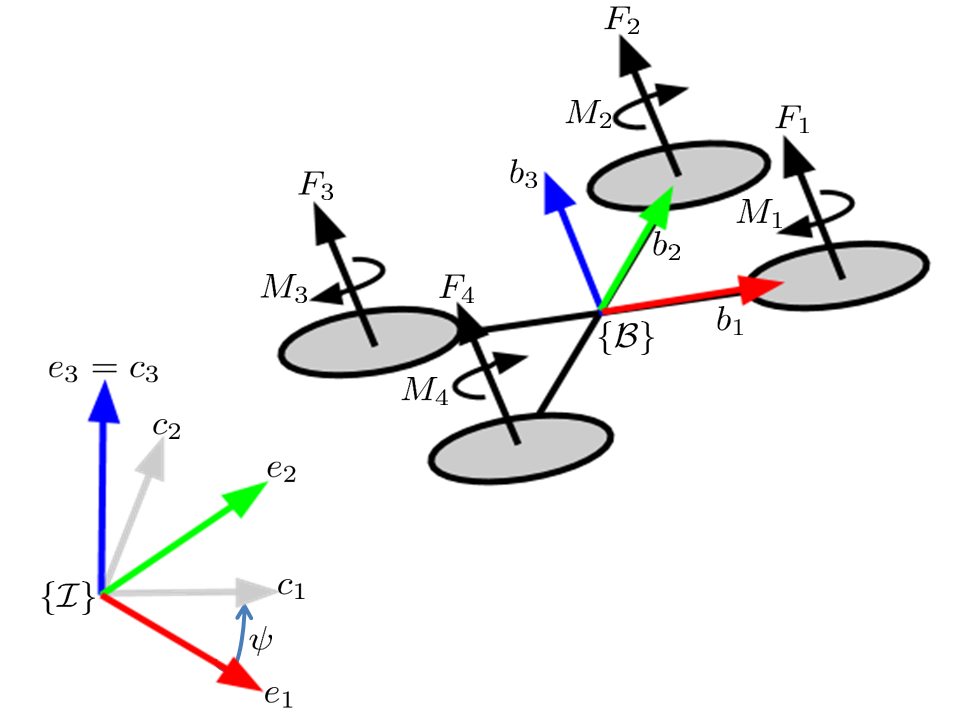
\includegraphics[width=.45\textwidth]{./StyleStuff/qrmodelppt.png}}
	\caption{Quadrotor-Load model representation\label{fig:mod.modelQRtrad}}
\end{figure}

The unit vector $ q $ from the \a{qr} to the load is represented in \BF. Define $ \phi_L $ as the yaw-rotation of the load around the z-axis of \BF and $ \theta_L $ as the angle between the cable and the z-axis of \BF, see Figure \ref{fig:mod.modelQRLtrad}.
\begin{figure}[h!]
	%ADD figure with angles phiL and theta L
	\centering
	\makebox[\textwidth][c]{\includegraphics[width=.45\textwidth]{./StyleStuff/dcsc.png}}
	\caption{\label{fig:mod.modelQRLtrad}}
\end{figure}	

\begin{equation}\label{eq:q}
%		q=-R_{\psi_L}R_{\theta_L}e_3=\begin{bmatrix}
%		s_{\theta_L}c_{\psi_L}\\s_{\theta_L}s_{\psi_L}\\-c_{\theta_L}
%		\end{bmatrix}
%\begin{align}
q=\begin{bmatrix}
s_{\theta_L}c_{\phi_L}\\
s_{\theta_L}s_{\phi_L}\\
c_{\theta_L}
\end{bmatrix}
%\dot{q}&=\begin{bmatrix}
%s_{\theta_L}c_{\psi_L}\\
%s_{\theta_L}s_{\psi_L}\\
%c_{\theta_L}
%\end{bmatrix}\\
%\end{align}
\end{equation}  
Differentiating Equation (\ref{eq:xQ2xL}) and (\ref{eq:q}) gives
\begin{equation}\label{key}
\begin{aligned}
\ddot{x}_L&=\ddot{x}_Q-\ddot{q}L\\
\ddot{q}&=\begin{bmatrix}
\ddot{\theta}_Lc_{\theta_L}c_{\phi_L}-\ddot{\phi}_Ls_{\theta_L}s_{\phi_L}-\dot{\phi}_L^2s_{\theta_L}c_{\phi_L}-\dot{\theta}_L^2s_{\theta_L}c_{\phi_L}-2\dot{\theta}_L\dot{\phi}_Lc_{\theta_L}s_{\phi_L}\\
\ddot{\theta}_Lc_{\theta_L}s_{\phi_L}+\ddot{\phi}_Ls_{\theta_L}c_{\phi_L}-\dot{\phi}_L^2s_{\theta_L}s_{\phi_L}-\dot{\theta}_L^2s_{\theta_L}s_{\phi_L}+2\dot{\theta}_L\dot{\phi}_Lc_{\theta_L}c_{\phi_L}\\
-\ddot{\theta}_Ls_{\theta_L}-\dot{\theta}_L^2 c_{\theta_L}\\
\end{bmatrix}
\end{aligned}
\end{equation}

\begin{equation}\label{key}
\begin{aligned}
\ddot{x}_Q&=\frac{1}{m_Q}(f(c_{\psi}s_{\theta}+c_{\theta}s_{\phi}s_{\psi})-Ts_{\theta_L}c_{\psi_L})\\
\ddot{y}_Q&=\frac{1}{m_Q}(f(s_{\psi}s_{\theta}-c_{\psi}c_{\theta}s_{\phi})-Ts_{\theta_L}s_{\psi_L})\\
\ddot{z}_Q&=\frac{1}{m_Q}(f(c_{\phi}c_{\theta})-Tc_{\theta_L})-g\\
\end{aligned}
\end{equation}



\begin{align}\label{key}
%CHECK wat is hier de bedoeling van? Checken in Garcia of literatuur?
	\ddot{\psi}&=\tilde{\tau}_{\psi}\\
\ddot{\theta}&=\tilde{\tau}_{\theta}\\
\ddot{\phi} &=\tilde{\tau}_{\phi}
\end{align}

\section{Summary}

***************************************\\
Compact, unambiguous, globally defined, 

Pro/Cons of Classical Modeling Techniques vs Geometric Modeling\\

Linearized model/State Space model vs. Geometric modeling\\


Geometric Mechanics/Lie Groups/Lie Algebra is used in order to represent the dynamics of the system onto the nonlinear configuration manifold $ SE(3) $\\
Advantage of this method is\\
Enables to model on \\
That type of control is discussed in the next chapter


***************************************\\